\documentclass[11pt]{article}
\usepackage[utf8]{inputenc}
\usepackage[czech]{babel}
\usepackage{a4wide}
\usepackage{amsmath}
\usepackage{graphicx}

\usepackage[pdfborder=0 0 0]{hyperref}



\title{Základy Počítačové grafiky}
\author{Tomáš Maršálek}
\date{27.\,října 2012}



\begin{document}
\maketitle
\section{Úvod}
Pro semestrální práci jsem po osobní dohodě se cvičícím zvolil jazyk Java, poté
podle vlastního výběru jeden z nejpoužívanějších wrapperů OpenGL pro Javu -
\textbf {Lightweight Java Game Library (LWJGL)}.


\section{Výpočty}
\subsection{Terén}
Terén je načten ze souboru a v programu používán jako objekt třídy
\textbf{Terrain}. Terén je $H - 1$ trojúhelníkových pruhů
(\textit{GL\_TRIANGLE\_STRIPS}) délky $W$. Objekt \textbf{Terrain} ulehčuje
práci pomocí metod umožňujících získání výšky nebo normály v daném bodě
této trojúhelníkové sítě.

\subsection{Výpočet normál terénu}
Normála v každém bodě trojúhelníkové sítě je vypočtena jako průměr normál čtyř
okolních myšlených trojúhelníků, popřípadě tří normál na hraně terénu nebo dvou
v rozích. Výsledek je pak znormalizován na jednotkovou velikost. \\

\begin{align*}
\mathbf {n1} &= \left[ \mathbf {terrain}(x + 1, z) - \mathbf {terrain}(x, z)
\right] \times \left[ \mathbf {terrain}(x, z + 1) - \mathbf {terrain}(x, z)
\right] \\
%
\mathbf {n2} &= \left[ \mathbf {terrain}(x, z + 1) - \mathbf {terrain}(x, z)
\right] \times \left[ \mathbf {terrain}(x - 1, z) - \mathbf {terrain}(x, z)
\right] \\
%
\mathbf {n3} &= \left[ \mathbf {terrain}(x - 1, z) - \mathbf {terrain}(x, z)
\right] \times \left[ \mathbf {terrain}(x, z - 1) - \mathbf {terrain}(x, z)
\right] \\
%
\mathbf {n4} &= \left[ \mathbf {terrain}(x, z - 1) - \mathbf {terrain}(x, z)
\right] \times \left[ \mathbf {terrain}(x + 1, z) - \mathbf {terrain}(x, z)
\right] \\
\end{align*}

\begin{align*}
\mathbf n &:= \mathbf {n1} + \mathbf {n2} + \mathbf {n3} + \mathbf {n4} \\
\mathbf n &:= \frac{\mathbf n}{\|\mathbf n\|} \\
\end{align*}

\begin{figure}[ht!]
\centering
	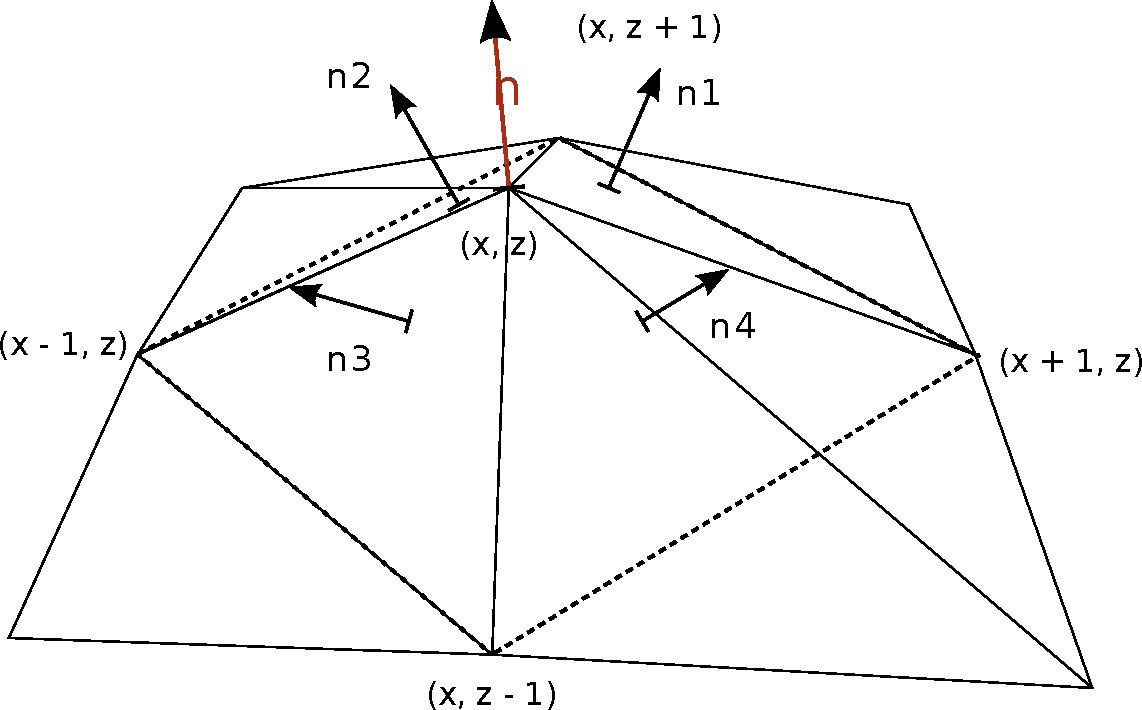
\includegraphics[width=10cm]{normals_persp.pdf}
	\caption{výpočet normály vrcholu}
\end{figure}

\subsection{Detekce kolizí při pohybu po terénu}
Pro detekci kolizí slouží metoda $float~getY(x, z)$, která vypočte y-souřadnici
nad pozicí (x, z) v rovině.

\subsubsection{getY}
Body x a z se zaokrouhlí dolů, tedy získáme souřadnice nejbližšího rohu čtverce
směrem doleva dolů, tzn. bodu $\mathbf a$.

Jestliže víme, ve kterém čtverci sítě terénu se nacházíme, musíme ještě
rozhodnout ze dvou trojúhelníků tohoto čtverce. Skalární součin vektoru s
rovinnou normálou vektoru $\mathbf b - \mathbf c$ určuje v rovině XZ
polorovinu, podle znaménka výsledku, čímž zjistíme onen trojúhelník.  
$$
(\mathbf
c - \mathbf b) \cdot \mathbf n = 0
$$
$$
sign(\mathbf n \cdot \mathbf x) = polorovina
$$


\begin{figure}[ht!]
\centering
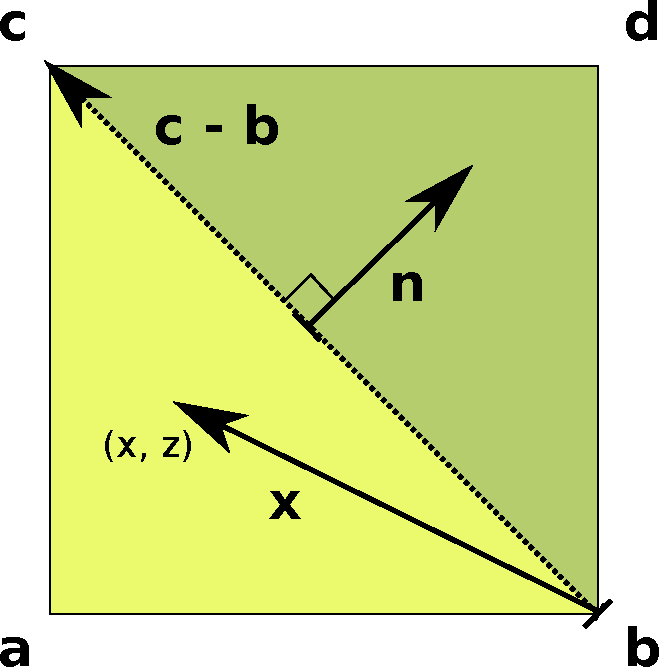
\includegraphics[width=8cm]{triangl.pdf}
	\caption{Rozdělení čtverce na poloroviny}
\end{figure}

Jestliže známe trojúhelník, můžeme vypočítat kýženou y-souřadnici nad bodem (x,
z). Rovinu, ve které trojúhelník leží definujeme alespoň jedním bodem
trojúhelníku a normálou trojúhelníka. Normálu získáme vektorovým součinem
libovolných dvou jeho hran. U normály $\mathbf n$ nezáleží ani na velikosti ani
na orientaci. Rovina splňuje rovnici $\mathbf n \cdot (\mathbf x - \mathbf a) =
0$, kde vektor $\mathbf x$ je pozice bodu od počátku a $\mathbf a$ je pozice
jednoho z bodů na trojúhelníku. Y získáme jednoduše jako řešení této rovnice.

\begin{align*}
\mathbf n \cdot (\mathbf x - \mathbf a) &= 0 \\
\mathbf n \cdot \mathbf x &= \mathbf n \cdot \mathbf a \\
n_x x_x + n_y x_y + n_z x_z &= \mathbf n \cdot \mathbf a \\
x_y &= \frac{\mathbf n \cdot \mathbf a - n_x x_x - n_z x_z}{n_y} \\
\end{align*}

\subsubsection{Rychlostní vektor}
Poté je spočten směrový vektor v rovině XZ podle momentálně stisknutých
kláves WSAD. Výšková složka tohoto vektoru je dopočtena jako rozdíl výšky v
terénu nad současnou pozicí a výškou nad novou pozicí určenou směrovým vektorem
v rovině. Vektor je pak normalizován a zvětšen rychlostním koeficientem, který
zaručuje, že rychlost bude konstantně 3m/s nehledě na snímkové frekvenci.

Tento rychlostní vektor je pak přičten k současné pozici.

Problém však nastává s výškou pozorovatele nad terénem, která je pevně dána na
1.85m. Použitím relativního vektoru rychlosti dochází ke kumulaci
zaokrouhlovacích chyb a po chvíli chození po terénu je výška očí zcela jiná,
než 1.85m. Proto je v každém snímku provedena korekce, která zaručuje, že oči
budou neustále stejně vysoko.

\subsection{Plynulá intenzita světla}
Máme-li den, který trvá od času 0 (00:00) do 1 (24:00), očekáváme v čase 0.5
nejvyšší intenzitu světla. Použitá funkce určující intenzitu slunce je Gaussova
křivka centrovaná do bodu 0.5.
$$
Intenzita~=~e^{- (C(t - \frac{1}{2}))^2}
$$
kde C je magická konstanta, která byla nalezena po chvíli testování tak, aby
byl výsledek co nejbližší skutečnosti.

Získaná intenzita se používá přímo jako intenzita hlavního zdroje světla - slunce a jako barva atmosféry.

\clearpage
\section{Přeložení a spuštění}
Aplikace byla vyvíjena pod GNU/Linux, přiložené knihovny a instrukce pro
spuštění aplikace jsou pro Windows. Verze Javy je 1.6.

V kořenovém adresáři jsou dodatečně přiloženy spustitelné soubory vytvořené
pomocí utility \textbf{jarsplice}, které obsahují všechny potřebné knihovny a
nativní soubory.
\begin{itemize}
	\item \textbf{ZPG.exe} pro Windows
	\item \textbf{ZPG.sh} pro Linux
	\item \textbf{ZPG.jar} pro Windows i Linux, spuštění přes příkaz java -jar
\end{itemize}

\subsection{Z příkazové řádky}
spuštění přiloženého archivu:
\begin{verbatim}
bin$  java -jar ZPG_A10B0632P.jar
\end{verbatim}

\subsubsection{Přeložení ze zdrojového kódu přímo}
přeložení:
\begin{verbatim}
$  javac -d . -cp lib\jars\lwjgl.jar:lib\jars\lwjgl_util.jar; src\Main.java
src\Terrain.java
\end{verbatim}
spuštění:
\begin{verbatim}
$  java -cp lib\jars\lwjgl.jar;lib\jars\lwjgl_util.jar; Main
\end{verbatim}


\subsection{Použitím Ant}
Pokud je nainstalovaný Apache Ant, pak pro přeložení a spuštění stačí použít příkaz z adresáře obsahující skript \textit{build.xml}.
\begin{verbatim}
$  ant
\end{verbatim}
nebo 
\begin{verbatim}
$  ant run
\end{verbatim}

\subsection{V Eclipse}
Získání a integrace \textbf {LWJGL} pod eclipse je popsána ve videu
\cite{installtut}, ale není třeba. Práce je odevzdána přímo jako projekt
eclipse, tedy stačí v Eclipse importovat existující projekt. Při importu se
však smaže adresář bin, je třeba ho nakopírovat zpátky, jinak chybí soubor s
terénem v bin/data.


\section{Ovládání hry}
Kamerou pohneme standardně klávesami WSAD a otočíme pohybem myši. Invertování
vertikálního pohledu provedeme pomocí klávesy U a přepnutí mezi drátěným a
plným modelem pomocí klávesy C. Hru ukončíme stiskem klávesy ESC.


\begin{thebibliography}{3}
\bibitem[1]{rocks}
{\em Bill Jacobs} \\
{\bf OpenGL tutorial}
	2007 - 2012 \\
\url{http://www.videotutorialsrock.com/}

\bibitem[2]{installtut}
{\em TheCodingUniverse} \\
{\bf \#1 LWJGL Workspace - LWJGL Tutorials} \\
	2011 \\
\url{http://youtu.be/0v56I5UWrYY}

\bibitem[3]{wikistrips}
{\em Wikipedia contributors} \\
{\bf ``Triangle strip,'' Wikipedia, The Free Encyclopedia} \\
	(accessed October 27, 2012) \\
\url{http://en.wikipedia.org/wiki/Triangle_strip}


\end{thebibliography}

\end{document}
